\begin{figure}[H]
    \centering
    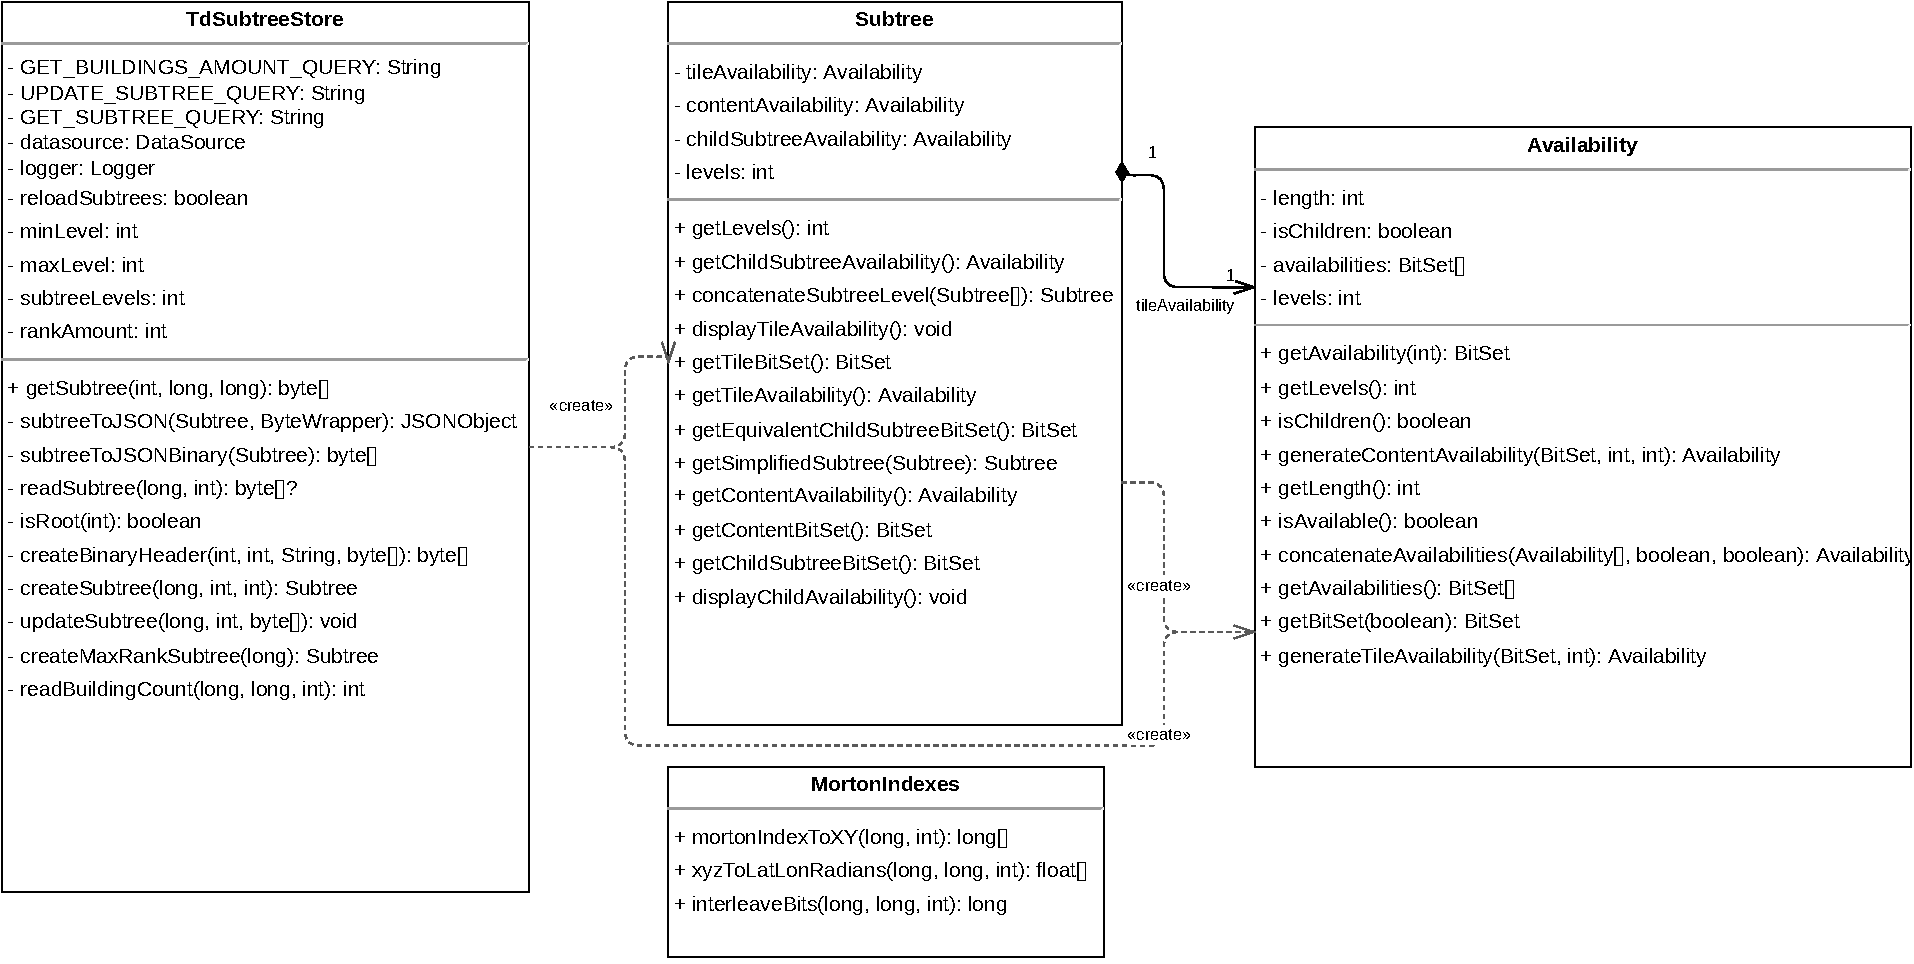
\includegraphics[width=1\textwidth]{assets/figures/subtree-classes.drawio.pdf}
    \caption{Classes utilisées pour la création d'une hiérarchie de Subtrees}
    \label{fig:subtree-classes}
\end{figure}

\subsection*{Classe Subtree}
\label{sec:subtree-class}

La première classe écrite dans le but de gérer les Subtrees est la classe \texttt{Subtree}. Un objet de cette classe comporte tout les éléments nécessaires pour la gestion d'un Subtree. Il contient un objet \texttt{Availability} pour chaque type de disponibilité (tuile, contenu, enfants) ainsi que le nombre de levels contenu. La classe offre aussi tous les getters utiles pour accéder aux informations importantes. Elle fournit aussi une fonction statique de concaténation de 4 Subtrees en un d'ordre supérieur. Cette fonction sera utilisée pour la création de l'arbre de Subtrees. Finalement, elle offre deux fonction de debug pour afficher les \textit{Tile Availability} et le \textit{Child Availability} dans la console.

\subsection*{Classe Availability}
\label{sec:availability-class}

La classe Availability est celle qui se chargera de stocker les listes de disponibilités. Pour cela, elle utilise un \textit{BitSet} par soucis d'optimisation. Tout comme la classe Subtree, elle offre une fonction de concaténation de 4 \textit{Availability} en une seule. De plus, elle propose deux fonctions pour générer un Availability complet à partir d'un BitSet représentant le dernier level du Subtree.

\subsection*{Classe TdSubtreeStore}
\label{sec:tdsubtreestore-class}

Cette classe est celle qui orchestrera la création et la distribution des Subtrees. Ce processus suit le diagramme suivant :

\begin{figure}[H]
    \centering
    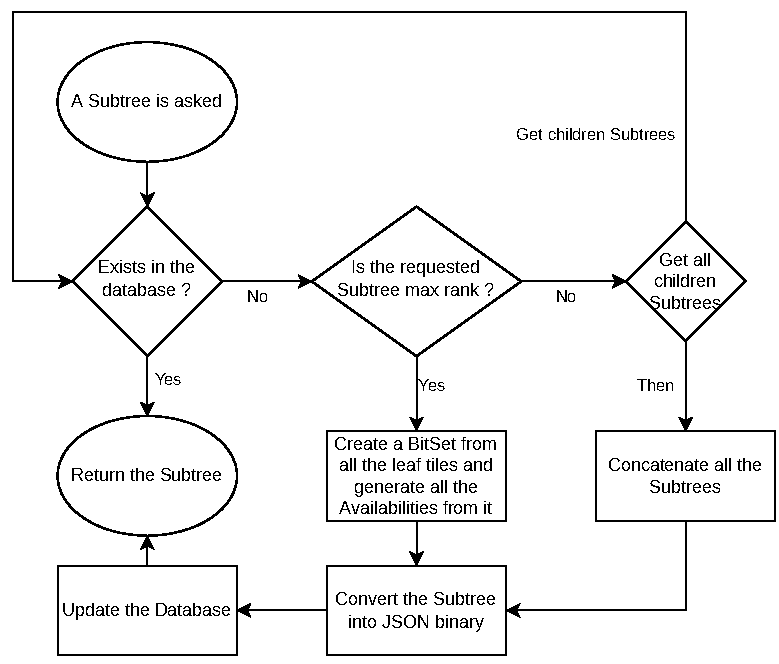
\includegraphics[width=1\textwidth]{assets/figures/simple-flowchart.drawio.pdf}
    \caption{Classes utilisées pour la création d'une hiérarchie de Subtrees}
    \label{fig:ssimple-flowchart}
\end{figure}

Vous observerez que la classe utilise un système récursif pour la création d'un Subtree. Puisqu'un Subtree parent doit être au courant des disponibilités des Subtrees enfants, il faudrait en théorie que ces derniers soient connus. Cependant, cela peut être optimisé en ne faisant que regarder si des bâtiments se trouvent dans la tuile enfant. Pour cela, une simple requête SQL simple permet de le déterminer :

\begin{verbatim}
SELECT EXISTS (
    SELECT 1
    FROM osm_ways
    WHERE (tags ? 'building' OR tags ? 'building:part')
    AND st_intersects(geom, st_makeenvelope(%1$s, %2$s, %3$s, %4$s, 4326))
) OR EXISTS (
    SELECT 1
    FROM osm_relations
    WHERE (tags ? 'building' OR tags ? 'building:part')
    AND st_intersects(geom, st_makeenvelope(%1$s, %2$s, %3$s, %4$s, 4326))
) AS has_buildings
\end{verbatim}

La différence de temps est significative :

\begin{listing}[h]
    
\end{listing}

Les deux méthodes ont des avantages et des inconvénients. La méthode calculant tous les Subtrees est énormément plus lente, mais les utilisateurs n'auront pas de temps d'attente supplémentaire lorsqu'ils se déplaceront dans la carte. La méthode calculant les Subtrees au fur et à mesure est quasiment instantanée, mais les utilisateurs devront attendre un peu plus longtemps lorsqu'ils se déplaceront dans la carte.

Pour le développement de l'application, je recommande donc de ne pas calculer tous les Subtrees en avance car il y en a rarement besoins. Par contre, pour un usage en production, il serait préférable de les calculer en avance.

Ce choix ainsi que le choix de re-créer les Subtrees ou les fichiers glTF des tuiles peuvent être modifiés dans la classe \texttt{TdTilesResources}\footnote{org/apache/baremaps/server/TdTilesResources.java}.